% Optics Ray Diagrams
% Demonstrates: converging/diverging lens ray tracing, mirrors, focal points.
% Compile with: pdflatex main.tex

\documentclass[border=10pt]{standalone}
\usepackage{tikz}
\usetikzlibrary{arrows.meta, decorations.markings, calc}

\begin{document}
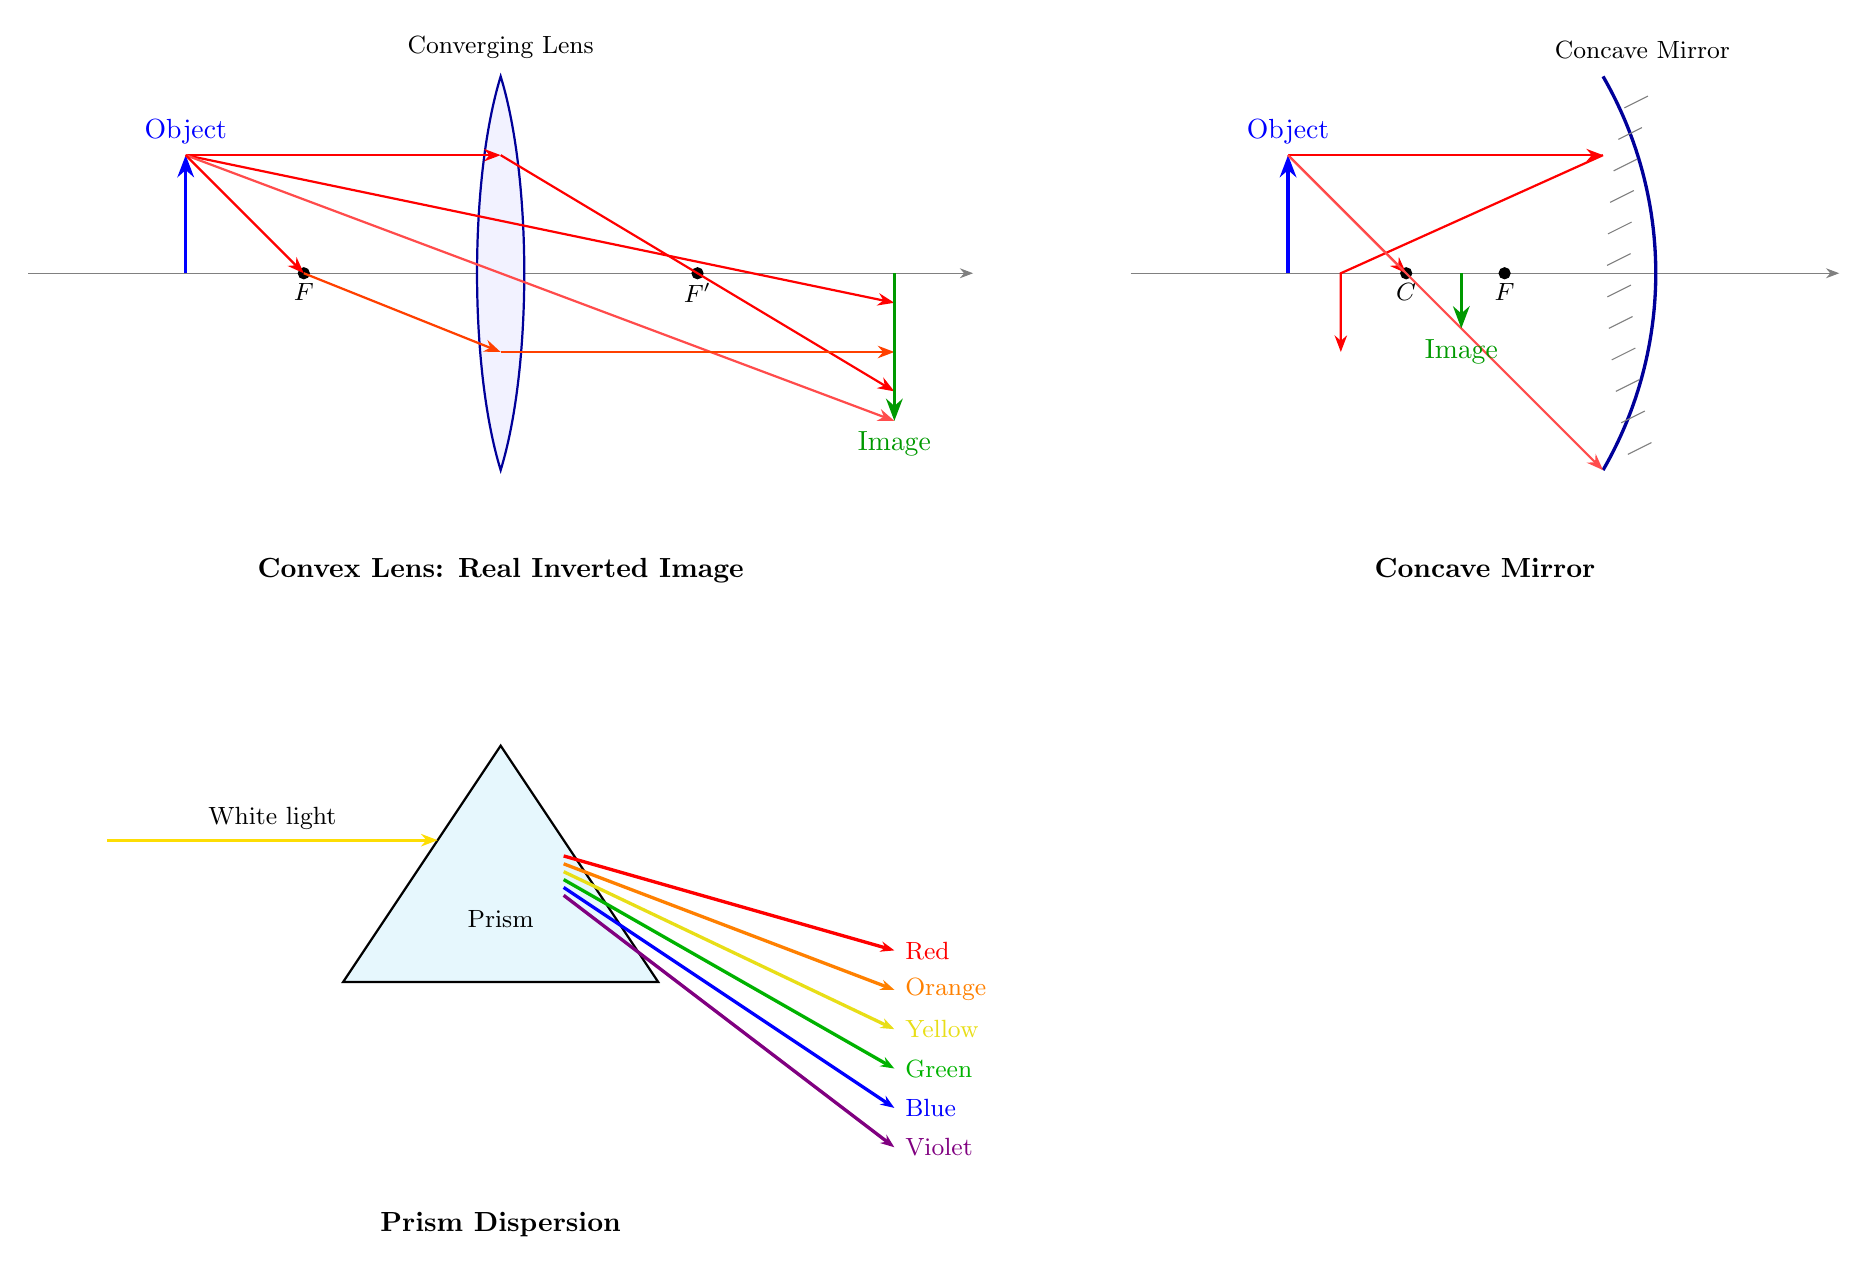
\begin{tikzpicture}[
    >=Stealth,
    ray/.style={thick, red, -{Stealth[length=6pt]}},
    virtual/.style={thick, red, dashed, -{Stealth[length=6pt]}},
    object/.style={very thick, blue, -{Stealth[length=8pt]}},
    image/.style={very thick, green!60!black, -{Stealth[length=8pt]}},
]

% =============================================================================
% Scene 1: Converging (convex) lens — real image
% =============================================================================
\begin{scope}[shift={(0,0)}]

    % --- Optical axis ---
    \draw[gray, thin, ->] (-6, 0) -- (6, 0) node[right] {};

    % --- Lens (double convex) ---
    \draw[thick, blue!60!black, fill=blue!5]
        (0, -2.5) .. controls (0.4, -1.2) and (0.4, 1.2) .. (0, 2.5)
        .. controls (-0.4, 1.2) and (-0.4, -1.2) .. cycle;
    \node[above, font=\small] at (0, 2.6) {Converging Lens};

    % --- Focal points ---
    \filldraw (2.5, 0) circle (2pt) node[below, font=\small] {$F'$};
    \filldraw (-2.5, 0) circle (2pt) node[below, font=\small] {$F$};

    % --- Object (arrow) ---
    \draw[object] (-4, 0) -- (-4, 1.5) node[above] {Object};

    % --- Three principal rays ---
    % Ray 1: Parallel to axis → through F'
    \draw[ray] (-4, 1.5) -- (0, 1.5);
    \draw[ray] (0, 1.5) -- (5, {1.5 - 1.5/2.5 * 5});

    % Ray 2: Through center → straight
    \draw[ray] (-4, 1.5) -- (5, {1.5 * (5+4)/4 * (-1) + 1.5 + 1.5});
    % Simplified: through (0,0) lens center
    \draw[ray, red!70] (-4, 1.5) -- (5, {-1.5/4 * 5});

    % Ray 3: Through F → parallel after lens
    \draw[ray] (-4, 1.5) -- (-2.5, 0);
    \draw[ray, red!50!orange] (-2.5, 0) -- (0, {-1.5/1.5*2.5 + 1.5});
    % Simplify: goes to lens then parallel
    \draw[ray, red!50!orange] (0, -1) -- (5, -1);

    % --- Image (inverted arrow) ---
    \coordinate (img) at ($(0,0)!1.66!(0, {-1.5*2.5/1.5})$);
    \draw[image] (5, 0) -- (5, -1.875) node[below] {Image};

    \node[font=\bfseries, anchor=north] at (0, -3.5) {Convex Lens: Real Inverted Image};
\end{scope}

% =============================================================================
% Scene 2: Concave mirror — real image
% =============================================================================
\begin{scope}[shift={(14, 0)}]

    % --- Optical axis ---
    \draw[gray, thin, ->] (-6, 0) -- (3, 0);

    % --- Concave mirror (arc) ---
    \draw[very thick, blue!60!black]
        (0, -2.5) arc[start angle=-30, end angle=30, radius=5];
    % Hatching behind mirror
    \foreach \y in {-2.3,-1.9,...,2.3} {
        \draw[gray, thin] ({0.05+0.05*\y*\y}, \y) -- ++(0.3, 0.15);
    }
    \node[above, font=\small] at (0.5, 2.6) {Concave Mirror};

    % --- Center of curvature and focal point ---
    \filldraw (-2.5, 0) circle (2pt) node[below, font=\small] {$C$};
    \filldraw (-1.25, 0) circle (2pt) node[below, font=\small] {$F$};

    % --- Object ---
    \draw[object] (-4, 0) -- (-4, 1.5) node[above] {Object};

    % --- Ray 1: Parallel → reflects through F ---
    \draw[ray] (-4, 1.5) -- (0, 1.5);
    \draw[ray] (0, 1.5) -- (-3.33, 0) -- (-3.33, -1);

    % --- Ray 2: Through C → reflects back on itself ---
    \draw[ray] (-4, 1.5) -- (-2.5, {1.5*(2.5-2.5)/(4-2.5)});
    \draw[ray, red!70] (-4, 1.5) -- (0, {1.5*(-0+4)/(4-2.5)*(-1)+1.5});

    % Simplified approach: just show the image
    \draw[image] (-1.8, 0) -- (-1.8, -0.7) node[below] {Image};

    \node[font=\bfseries, anchor=north] at (-1.5, -3.5) {Concave Mirror};
\end{scope}

% =============================================================================
% Scene 3: Prism dispersion
% =============================================================================
\begin{scope}[shift={(0, -9)}]

    % --- Prism ---
    \coordinate (A) at (0, 3);
    \coordinate (B) at (-2, 0);
    \coordinate (C) at (2, 0);

    \filldraw[fill=cyan!10, draw=black, thick] (A) -- (B) -- (C) -- cycle;
    \node[font=\small] at (0, 0.8) {Prism};

    % --- Incident white light ---
    \draw[very thick, yellow!80!orange, -{Stealth[length=6pt]}]
        (-5, 1.8) -- (-0.8, 1.8) node[midway, above, font=\small, text=black] {White light};

    % --- Refracted / dispersed rays ---
    \draw[very thick, red, -{Stealth[length=5pt]}]
        (0.8, 1.6) -- (5, 0.4) node[right, font=\small] {Red};
    \draw[very thick, orange, -{Stealth[length=5pt]}]
        (0.8, 1.5) -- (5, -0.1) node[right, font=\small] {Orange};
    \draw[very thick, yellow!90!black, -{Stealth[length=5pt]}]
        (0.8, 1.4) -- (5, -0.6) node[right, font=\small] {Yellow};
    \draw[very thick, green!70!black, -{Stealth[length=5pt]}]
        (0.8, 1.3) -- (5, -1.1) node[right, font=\small] {Green};
    \draw[very thick, blue, -{Stealth[length=5pt]}]
        (0.8, 1.2) -- (5, -1.6) node[right, font=\small] {Blue};
    \draw[very thick, violet, -{Stealth[length=5pt]}]
        (0.8, 1.1) -- (5, -2.1) node[right, font=\small] {Violet};

    \node[font=\bfseries, anchor=north] at (0, -2.8) {Prism Dispersion};
\end{scope}

\end{tikzpicture}
\end{document}
